\textit{Feedforward neural networks} or \textit{multilayer perceptrons} (MLPs) are the essential deep learning models. A feedforward neural network defines a mapping $f (\pmb{x} ; \pmb{\theta}) = \pmb{y}$ and learns the value of the parameters $\pmb{\theta}$ that result in the best function approximation.

A neural network consists of several \textit{layers}. There is always one \textit{input} layer, followed by one or more \textit{hidden} layers and finally, there is an \textit{output layer}. The number of layers (without the input layer) defines the \textit{depth} of the model. There is no precise definition, but neural networks with more than three layers are called \textit{deep} neural networks. 

When it comes to feedforward neural networks, a network is a directed acyclic graph. Vertices of such a graph are called \textit{units} or \textit{neurons} and edges are called \textit{weights}. Vertices represent scalar functions of an input. Weights are the parameters $\pmb \theta$ which a neural network learns. Edges define data flow. One example of such a model is shown in the Figure \ref{fig:basic-cnn}.


\begin{figure}
\centering
\def\layersep{2.5cm}
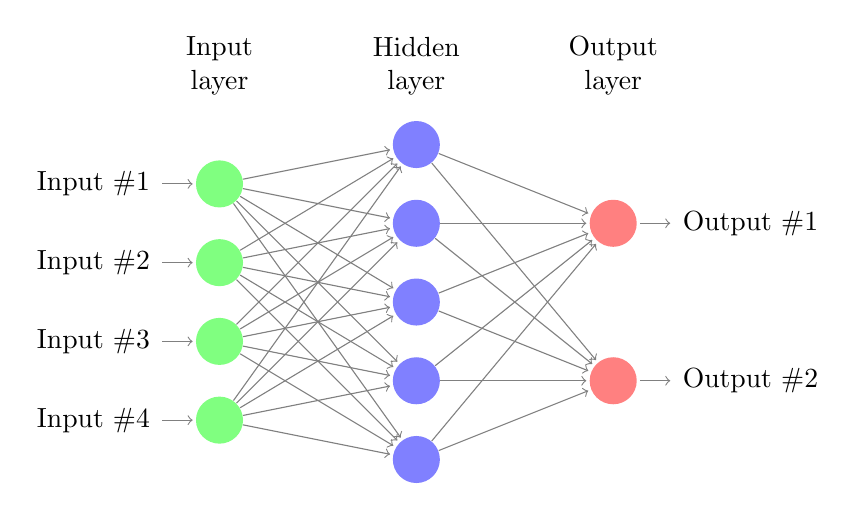
\begin{tikzpicture}[shorten >=1pt,->,draw=black!50, node distance=\layersep]
    \tikzstyle{every pin edge}=[<-,shorten <=1pt]
    \tikzstyle{neuron}=[circle,fill=black!25,minimum size=17pt,inner sep=0pt]
    \tikzstyle{input neuron}=[neuron, fill=green!50];
    \tikzstyle{output neuron}=[neuron, fill=red!50];
    \tikzstyle{hidden neuron}=[neuron, fill=blue!50];
    \tikzstyle{annot} = [text width=4em, text centered]

    % Draw the input layer nodes
    \foreach \name / \y in {1,...,4}
    % This is the same as writing \foreach \name / \y in {1/1,2/2,3/3,4/4}
        \node[input neuron, pin=left:Input \#\y] (I-\name) at (0,-\y) {};

    % Draw the hidden layer nodes
    \foreach \name / \y in {1,...,5}
        \path[yshift=0.5cm]
            node[hidden neuron] (H-\name) at (\layersep,-\y cm) {};

    % Draw the output layer node
    \node[output neuron,pin={[pin edge={->}]right:Output \#1}, right of=H-2] (OO) {};
    \node[output neuron,pin={[pin edge={->}]right:Output \#2}, right of=H-4] (OT) {};


    % Connect every node in the input layer with every node in the
    % hidden layer.
    \foreach \source in {1,...,4}
        \foreach \dest in {1,...,5}
            \path (I-\source) edge (H-\dest);

    % Connect every node in the hidden layer with the output layer
    \foreach \source in {1,...,5}
        \path (H-\source) edge (OO);
    \foreach \source in {1,...,5}
        \path (H-\source) edge (OT);

    % Annotate the layers
    \node[annot,above of=H-1, node distance=1cm] (hl) {Hidden layer};
    \node[annot,left of=hl] {Input layer};
    \node[annot,right of=hl] {Output layer};
\end{tikzpicture}

\caption{An example of the feedforward neural network architecture}
\label{fig:basic-cnn}
\end{figure}


A typical architecture of one neuron can be seen in the Figure \ref{fig:basic-neuron}. That specific neuron performs an operation $ f(net) = y $ where $net = x1*w1 + x2*w2 + x3*w3 + bias$.  Bias is usually modelled as an additional input with the corresponding weight $w=1$. Then a neuron performs the operation $ f(\pmb x \times \pmb w) = y$ where $\times$ denotes cross-product between two vectors. Function $f$ is called an \textit{activation function} and usually is the same for all neurons in the same layer. In the input layer the activation function is mapping from input to output, i.e. $f(x) = x$, but those in the other layers are usually non-linear functions. 

Usually we are interested in \textit{probabilities} for every class, i.e. what's the probability that a given sample belongs to a specific class. In that case, we want a vector of the probabilities as an output of a neural network. If there are $N$ different classes, the vector will have dimensionality of $N$. The sum of the probabilities for all classes must be equal to $1$. Then, if we want to find out a predicted label for a given sample, we take the class that corresponds to the index with the highest probability. The layer that provides such a vector as an output is called \textit{softmax} layer and usually represents the last layer in a neural network that is used for classification. Sometimes the softmax layer is not even considered part of a neural network, but only as a function used for post-processing an output of a neural network. In this thesis, when it matters, it is clear from the context if the last layer is a softmax layer or not.

 \textit{Convolutional Neural Networks} (CNNs), which are described in Subsection \ref{subsection:convolutionalNN}, are a specific kind of feedforward neural networks. They are most popular in the computer vision domain. In domains where a context is important, for instance in Natural Language Processing, cycles are introduced in a computing graph so that the context can be stored in a state of a neural network.  The \textit{Recurrent Neural Networks} (RNNs) are an example of a neural network with cycles. However, RNNs are out of the scope of this thesis and will not be further discussed.

\begin{figure}
\begin{tikzpicture}[
init/.style={
  draw,
  circle,
  inner sep=2pt,
  font=\Huge,
  join = by -latex
},
squa/.style={
  draw,
  inner sep=2pt,
  font=\Large,
  join = by -latex
},
start chain=2,node distance=13mm
]
\node[on chain=2] 
  (x2) {$x_2$};
\node[on chain=2,join=by o-latex] 
  {$w_2$};
\node[on chain=2,init] (sigma) 
  {$\displaystyle\Sigma$};
\node[on chain=2,squa,label=above:{\parbox{2cm}{\centering Activation \\ function}}]   
  {$f$};
\node[on chain=2,label=above:Output,join=by -latex] 
  {$y$};
\begin{scope}[start chain=1]
\node[on chain=1] at (0,1.5cm) 
  (x1) {$x_1$};
\node[on chain=1,join=by o-latex] 
  (w1) {$w_1$};
\end{scope}
\begin{scope}[start chain=3]
\node[on chain=3] at (0,-1.5cm) 
  (x3) {$x_3$};
\node[on chain=3,label=below:Weights,join=by o-latex] 
  (w3) {$w_3$};
\end{scope}
\node[label=above:\parbox{2cm}{\centering Bias \\ $b$}] at (sigma|-w1) (b) {};

\draw[-latex] (w1) -- (sigma);
\draw[-latex] (w3) -- (sigma);
\draw[o-latex] (b) -- (sigma);

\draw[decorate,decoration={brace,mirror}] (x1.north west) -- node[left=10pt] {Inputs} (x3.south west);
\end{tikzpicture}
\caption{A single processing unit in a neural network}
\label{fig:basic-neuron}
\end{figure}